\documentclass{beamer}

\usepackage[utf8]{inputenc}
\usepackage[spanish]{babel}
\usepackage{amsmath}
\usepackage{amssymb}
\usepackage{tikz}
\usetikzlibrary{arrows,calc,positioning}
%\usetheme{Goddard}
\usetheme{Madrid}
\hypersetup{colorlinks,allcolors=.,urlcolor=magenta}
\usepackage{listings}
\lstset{
    language=Matlab,
    basicstyle=\ttfamily\footnotesize,
    breaklines=true,
    frame=single,
    columns=flexible
}

\title{Investigación de Operaciones II}
\subtitle{Unidad 3: Fundamentos de la Teoría de Colas}
\author[RL]{Ricardo Jesús Largaespada Fernández}
\institute[UNI]{Ingeniería de Sistemas, DACTIC, UNI}
\date{13 de Mayo, 2025}

\begin{document}

% ---------------------------------------------------------------
% TÍTULO Y AGENDA
% ---------------------------------------------------------------
\frame{\titlepage}

\begin{frame}{Agenda}
    \tableofcontents
\end{frame}

\section{Sesión 19}

\begin{frame}{Sesión 19}
\textbf{Tema:}
\begin{enumerate}
    \item Modelos de colas basados en el proceso de nacimiento muerte.
    \begin{itemize}
        \item Modelo M/M/s
        \item Modelo M/M/1/K
    \end{itemize}
\end{enumerate}

\textbf{Objetivo:}
\begin{itemize}
    \item Resolver problemas de sistemas de colas mediante los modelos M/M/s y M/M/1/K, determinando sus parámetros operacionales ($W_q, L_q, \rho$) para proponer mejoras en la eficiencia de sistemas de atención con capacidad finita e infinita.
\end{itemize}
\end{frame}

\begin{frame}{Proceso de nacimiento y muerte}
\begin{center}
\scalebox{0.55}{
\begin{tikzpicture}[->, >=stealth, thick, node distance=2.5cm]

% Estados
\node[circle, draw] (s0) {0};
\node[circle, draw, right of=s0] (s1) {1};
\node[circle, draw, right of=s1] (s2) {2};
\node[circle, draw, right of=s2] (s3) {3};
\node[right of=s3, node distance=1.7cm] (dots1) {$\cdots$};
\node[circle, draw, right of=dots1, node distance=1.7cm] (sn2) {$n\!-\!2$};
\node[circle, draw, right of=sn2] (sn1) {$n\!-\!1$};
\node[circle, draw, right of=sn1] (sn) {$n$};
\node[circle, draw, right of=sn] (snplus1) {$n\!+\!1$};
\node[right of=snplus1, node distance=1.7cm] (dots2) {$\cdots$};

% Flechas de nacimiento (bend left)
\draw[bend left=20] (s0) to node[above] {$\lambda_0$} (s1);
\draw[bend left=20] (s1) to node[above] {$\lambda_1$} (s2);
\draw[bend left=20] (s2) to node[above] {$\lambda_2$} (s3);
\draw (s3) -- (dots1);
\draw (dots1) -- (sn2);
\draw[bend left=20] (sn2) to node[above] {$\lambda_{n-2}$} (sn1);
\draw[bend left=20] (sn1) to node[above] {$\lambda_{n-1}$} (sn);
\draw[bend left=20] (sn) to node[above] {$\lambda_n$} (snplus1);
\draw (snplus1) -- (dots2);

% Flechas de muerte (bend right)
\draw[bend left=20] (s1) to node[below] {$\mu_1$} (s0);
\draw[bend left=20] (s2) to node[below] {$\mu_2$} (s1);
\draw[bend left=20] (s3) to node[below] {$\mu_3$} (s2);
\draw[bend left=20] (sn1) to node[below] {$\mu_{n-1}$} (sn2);
\draw[bend left=20] (sn) to node[below] {$\mu_n$} (sn1);
\draw[bend left=20] (snplus1) to node[below] {$\mu_{n+1}$} (sn);

\end{tikzpicture}
}
\end{center}
\caption{Diagrama de tasas del proceso de nacimiento y muerte}
\end{frame}

\begin{frame}{Modelos basados en procesos de nacimiento y muerte}
\justifying
Como se puede asignar cualquier valor no negativo a cada una de las tasas medias $\lambda_0$, $\lambda_1$, \ldots, y $\mu_1$, $\mu_2$, \ldots\ del proceso de nacimiento y muerte, se cuenta con una gran flexibilidad para modelar un sistema de colas. 

Los modelos que acaso sean los que más se usan en teoría de colas se basan directamente en este proceso. De acuerdo con los supuestos 1 y 2 (y la propiedad 4 de la distribución exponencial), se dice que estos modelos tienen \textbf{entradas de Poisson y tiempos de servicio exponencial}.

Los modelos difieren sólo en los supuestos sobre cómo cambian las $\lambda_n$ y las $\mu_n$ según el estado $n$.
\end{frame}

\begin{frame}{Análisis del proceso de nacimiento y muerte}
\justifying
Como consecuencia de los supuestos 1 y 2, el proceso de nacimiento y muerte es un tipo especial de \textbf{cadena de Markov de tiempo continuo}. 

Dado que las tasas $\lambda_n$ y $\mu_n$ son tasas medias del sistema (por la propiedad de la distribución exponencial), el diagrama de tasas (figura anterior) muestra las \textit{únicas transiciones posibles} del sistema, y la tasa media asociada a cada una de ellas.

\medskip
El análisis se simplifica si el sistema ha alcanzado una condición de \textbf{estado estable}, ya que estudiar la distribución en condición transitoria es más complejo y poco práctico.

\end{frame}

\begin{frame}{Análisis del proceso de nacimiento y muerte}
Consideramos el número de veces que el proceso entra o sale de un estado $n$ hasta tiempo $t$:
\begin{itemize}
    \item $E_n(t)$: número de veces que el proceso entra al estado $n$ hasta el tiempo $t$.
    \item $L_n(t)$: número de veces que el proceso sale del estado $n$ hasta el tiempo $t$.
\end{itemize}

Dado que las entradas y salidas se alternan, se cumple:
\[
\left| E_n(t) - L_n(t) \right| \leq 1
\]

Dividiendo entre $t$ y tomando el límite cuando $t \to \infty$ se obtiene:
\[
\left| \frac{E_n(t)}{t} - \frac{L_n(t)}{t} \right| \leq \frac{1}{t} \quad \Rightarrow \quad \lim_{t \to \infty} \left( \frac{E_n(t)}{t} - \frac{L_n(t)}{t} \right) = 0
\]
\end{frame}

\begin{frame}{Principio de tasa de entrada = tasa de salida}
\justifying
Si se dividen $E_n(t)$ y $L_n(t)$ entre $t$, se obtiene la \textbf{tasa real} (número de eventos por unidad de tiempo) a la que ocurren estos dos tipos de eventos. 

Cuando $t \to \infty$, se obtiene la \textbf{tasa media} (número esperado de eventos por unidad de tiempo):

\begin{align*}
\lim_{t \to \infty} \frac{E_n(t)}{t} &= \text{tasa media a la que el proceso entra al estado } n. \\
\lim_{t \to \infty} \frac{L_n(t)}{t} &= \text{tasa media a la que el proceso sale del estado } n.
\end{align*}

\medskip
Estos resultados conducen al siguiente principio clave:

\begin{block}{\centering Principio de tasa de entrada = tasa de salida}
Para cualquier estado $n$ ($n = 0, 1, 2, \dots$) del sistema: 
\[
\text{tasa media de entrada} = \text{tasa media de salida}.
\]
\end{block}
\end{frame}

\begin{frame}{Ecuaciones de balance en estado estable}
\justifying
La ecuación que expresa el principio de \textit{tasa de entrada = tasa de salida} se llama \textbf{ecuación de balance} del estado $n$. 

\medskip
Después de construir las ecuaciones de balance de todos los estados en términos de las probabilidades $P_n$ \textit{desconocidas}, se puede resolver este sistema (junto con la condición de normalización $\sum P_n = 1$) para obtener la distribución estacionaria del sistema.
\end{frame}

\begin{frame}{Tabla de ecuaciones de balance}
\centering
\renewcommand{\arraystretch}{1.6}
\begin{tabular}{|c|c|}
\hline
\textbf{Estado} & \textbf{Tasa de entrada = Tasa de salida} \\
\hline
$0$ & $\mu_1 P_1 = \lambda_0 P_0$ \\
$1$ & $\lambda_0 P_0 + \mu_2 P_2 = (\lambda_1 + \mu_1) P_1$ \\
$2$ & $\lambda_1 P_1 + \mu_3 P_3 = (\lambda_2 + \mu_2) P_2$ \\
$\vdots$ & $\vdots$ \\
$n{-}1$ & $\lambda_{n-2} P_{n-2} + \mu_n P_n = (\lambda_{n-1} + \mu_{n-1}) P_{n-1}$ \\
$n$ & $\lambda_{n-1} P_{n-1} + \mu_{n+1} P_{n+1} = (\lambda_n + \mu_n) P_n$ \\
$\vdots$ & $\vdots$ \\
\hline
\end{tabular}
\end{frame}

\begin{frame}{Resultados del proceso de nacimiento y muerte}
\justifying
Al aplicar recursivamente las ecuaciones de balance se obtiene:

\[
P_1 = \frac{\lambda_0}{\mu_1} P_0, \quad
P_2 = \frac{\lambda_1}{\mu_2} P_1 = \frac{\lambda_1 \lambda_0}{\mu_2 \mu_1} P_0, \quad
P_3 = \frac{\lambda_2}{\mu_3} P_2 = \frac{\lambda_2 \lambda_1 \lambda_0}{\mu_3 \mu_2 \mu_1} P_0, \quad \ldots
\]

\medskip
En general, se define el coeficiente:
\[
C_n = \frac{\lambda_{n-1} \lambda_{n-2} \cdots \lambda_0}{\mu_n \mu_{n-1} \cdots \mu_1}, \quad \text{para } n \geq 1, \quad \text{y se define } C_0 = 1.
\]

Entonces, las probabilidades de estado estable se expresan como:
\[
P_n = C_n P_0, \quad \text{para } n = 0, 1, 2, \dots
\]

\medskip
Aplicando la condición de normalización:
\[
\sum_{n=0}^\infty P_n = 1 \quad \Rightarrow \quad P_0 = \left( \sum_{n=0}^\infty C_n \right)^{-1}
\]
\end{frame}

\begin{frame}{Medidas de desempeño en estado estable}
\justifying
Una vez que se conocen las probabilidades en estado estable $P_n$, se pueden obtener las medidas clave del sistema:

\begin{itemize}
    \item Número esperado de clientes en el sistema:
    \[
    L = \sum_{n=0}^{\infty} n P_n
    \]
    
    \item Número esperado de clientes en la cola:
    \[
    L_q = \sum_{n=s}^{\infty} (n - s) P_n
    \]

    \item Tiempo esperado en el sistema y en la cola (Ley de Little):
    \[
    W = \frac{L}{\bar{\lambda}}, \quad
    W_q = \frac{L_q}{\bar{\lambda}}
    \]
\end{itemize}

donde $\bar{\lambda}$ es la tasa promedio de llegadas, dada por:
\[
\bar{\lambda} = \sum_{n=0}^{\infty} \lambda_n P_n
\]
\end{frame}

\begin{frame}{Modelos de colas basados BD}
\justifying
Gracias a la flexibilidad del proceso de nacimiento y muerte, se puede modelar una amplia variedad de sistemas de colas, asignando libremente las tasas $\lambda_n$ y $\mu_n$ según el estado del sistema.

\medskip
Los modelos más comunes en la teoría de colas (como M/M/1, M/M/s y M/M/1/K) se construyen a partir de este proceso, suponiendo:

\begin{itemize}
    \item Llegadas según un proceso de \textbf{Poisson} (entradas independientes y exponencialmente distribuidas).
    \item Tiempos de servicio \textbf{exponenciales}.
\end{itemize}

\medskip
Lo que distingue a cada modelo es cómo cambian las tasas $\lambda_n$ y $\mu_n$ con respecto al número de clientes $n$ en el sistema.

\begin{block}{¿Qué sigue?}
Presentaremos tres modelos fundamentales de sistemas de colas, todos como casos particulares del proceso de nacimiento y muerte.
\end{block}
\end{frame}

\begin{frame}{Modelo M/M/s}
\justifying
El modelo \textbf{M/M/s} describe un sistema con:
\begin{itemize}
    \item Llegadas según un proceso de Poisson, con tasa constante $\lambda$.
    \item Tiempos de servicio exponenciales con tasa $\mu$ por servidor.
    \item $s$ servidores trabajando en paralelo.
\end{itemize}

\medskip
Este modelo es un caso particular del proceso de nacimiento y muerte, donde:

\[
\lambda_n = \lambda \quad \text{(para todo $n \geq 0$)}
\]
\[
\mu_n = 
\begin{cases}
n\mu & \text{si } n \leq s, \\
s\mu & \text{si } n > s.
\end{cases}
\]

\medskip
\textbf{Condición de estabilidad:}
\[
\rho = \frac{\lambda}{s\mu} < 1
\]
Si esta condición se cumple, el sistema alcanza una distribución de estado estable, y se pueden aplicar las fórmulas generales para $P_n$, $L$, $L_q$, etc.

\end{frame}

\begin{frame}{Resultados del modelo M/M/1}
\justifying
Para el caso de un solo servidor ($s = 1$), el modelo M/M/1 se caracteriza por:
\[
\lambda_n = \lambda, \quad \mu_n = \mu \quad \text{para todo } n \geq 0
\]

\medskip
Los coeficientes $C_n$ se simplifican como:
\[
C_n = \left( \frac{\lambda}{\mu} \right)^n = \rho^n, \quad \text{donde } \rho = \frac{\lambda}{\mu}
\]

\medskip
Entonces:
\[
P_n = \rho^n P_0
\]

Usando la condición de normalización $\sum_{n=0}^{\infty} P_n = 1$:
\[
P_0 = \left( \sum_{n=0}^{\infty} \rho^n \right)^{-1} = (1 - \rho)
\]

\medskip
\textbf{Distribución de estado estable del M/M/1:}
\[
P_n = (1 - \rho)\rho^n, \quad \text{para } n = 0, 1, 2, \dots
\]
\end{frame}

\begin{frame}{Medidas de desempeño del modelo M/M/1}
\justifying

Dado que $P_n = (1 - \rho)\rho^n$, se puede calcular:

\medskip
\textbf{Número esperado de clientes en el sistema:}
\begin{align}
L =& \sum_{n=0}^{\infty} n(1 - \rho)\rho^n = (1-\rho)\rho \sum_{n=0}^{\infty} n\rho^{n-1} = (1-\rho)\rho\frac{d}{d\rho}\sum_{n=0}^\infty\rho^n\\
=&(1-\rho)\rho\frac{d}{d\rho}\left( \frac{1}{1-\rho}\right) =(1-\rho)\rho\cdot \frac{1}{(1-\rho)^2}= \frac{\rho}{1-\rho}=\frac{\lambda}{\mu - \lambda} 
\end{align}

\textbf{Número esperado de clientes en la cola:}
\[
L_q = \sum_{n=1}^{\infty} (n - 1)P_n = L - (1 - P_0) = \frac{\lambda^2}{\mu(\mu - \lambda)}
\]

\medskip
\textbf{Condición de estabilidad:} \( \lambda < \mu \)

\begin{block}{Advertencia}
Si $\lambda \geq \mu$, la suma para $P_0$ diverge. El sistema no alcanza estado estable y la cola crece indefinidamente.
\end{block}
\end{frame}

\begin{frame}{Diagrama de tasas del modelo M/M/s}
\justifying
El modelo M/M/s es un caso del proceso de nacimiento y muerte donde las tasas de servicio cambian según el número de servidores ocupados.

\begin{center}
    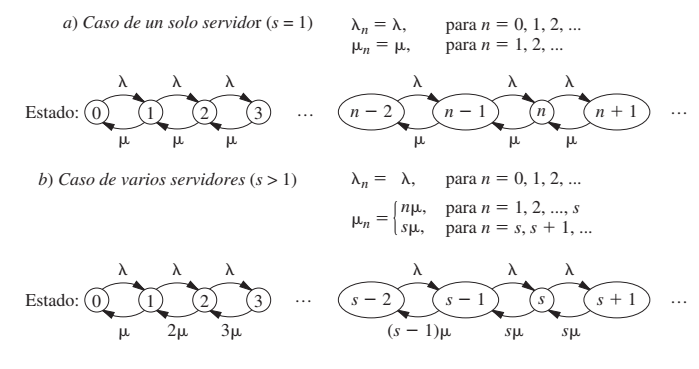
\includegraphics[width=0.9\textwidth]{images/Modelo_mms.png}
\end{center}
\end{frame}

\begin{frame}{Tiempos de espera en el modelo M/M/1}
\justifying
En el modelo M/M/1, el tiempo de espera \textbf{en el sistema} (incluye el servicio) sigue una distribución exponencial con parámetro $\mu(1 - \rho)$.

\medskip
\textbf{Tiempo esperado en el sistema:}
\[
W = \frac{1}{\mu(1 - \rho)} = \frac{1}{\mu - \lambda}
\]

\textbf{Tiempo esperado en la cola (excluye servicio):}
\[
W_q = \frac{\rho}{\mu(1 - \rho)} = \frac{\lambda}{\mu(\mu - \lambda)}
\]

\medskip
Estos resultados siguen de aplicar la ley de Little: $W = \frac{L}{\lambda}$ y $W_q = \frac{L_q}{\lambda}$.
\end{frame}

\begin{frame}{Resultados del modelo M/M/s (con $s > 1$)}
\justifying
\textbf{Condición de estabilidad: } $ \rho = \frac{\lambda}{s\mu} < 1 $. Cuando $s > 1$, los coeficientes $C_n$ del proceso de nacimiento y muerte se convierten en:
\[
C_n = 
\begin{cases}
\displaystyle \frac{(\lambda/\mu)^n}{n!} & \text{si } 1 \leq n \leq s \\[1.5ex]
\displaystyle \frac{(\lambda/\mu)^s}{s!} \cdot \left( \frac{\lambda}{s\mu} \right)^{n - s} = \frac{(\lambda/\mu)^n}{s! \cdot s^{n - s}} & \text{si } n \geq s
\end{cases}
\]

\medskip
\textbf{Probabilidad de estado vacío:}
\[
P_0 = \left[ \sum_{n=0}^{s-1} \frac{(\lambda/\mu)^n}{n!} + \frac{(\lambda/\mu)^s}{s!} \cdot \frac{1}{1 - \rho} \right]^{-1}
\]

\textbf{Distribución de estado:}
\[
P_n = 
\begin{cases}
\displaystyle \frac{(\lambda/\mu)^n}{n!} P_0 & \text{si } 0 \leq n \leq s \\[1.5ex]
\displaystyle \frac{(\lambda/\mu)^n}{s! \cdot s^{n - s}} P_0 & \text{si } n \geq s
\end{cases}
\]

\end{frame}

\begin{frame}{Cálculo de $L_q$, $W_q$, $W$ y $L$ en el modelo M/M/s}
\justifying
\textbf{Número esperado de clientes en la cola:}
\[
L_q = \sum_{n=s}^{\infty} (n - s)P_n
= \sum_{j=0}^{\infty} j P_{s+j}
= \sum_{j=0}^{\infty} j \cdot \frac{(\lambda/\mu)^s}{s!} \rho^j P_0
\]
\[
= P_0 \cdot \frac{(\lambda/\mu)^s}{s!} \cdot \rho \cdot \frac{d}{d\rho} \left( \sum_{j=0}^{\infty} \rho^j \right)
= \frac{P_0 (\lambda/\mu)^s \rho}{s! (1 - \rho)^2}
\]

\textbf{Tiempo de espera en la cola:}
\[
W_q = \frac{L_q}{\lambda}
\]

\textbf{Tiempo de espera en el sistema:}
\[
W = W_q + \frac{1}{\mu}
\]

\textbf{Número esperado de clientes en el sistema:}
\[
L = \lambda \cdot W = L_q + \frac{\lambda}{\mu}
\]
\end{frame}

\begin{frame}{Modelo M/M/s/K (cola finita)}
\justifying
El modelo \textbf{M/M/s/K} representa un sistema de colas con:

\begin{itemize}
    \item Llegadas de Poisson con tasa $\lambda$.
    \item Tiempos de servicio exponenciales con tasa $\mu$ por servidor.
    \item $s$ servidores disponibles.
    \item Capacidad máxima del sistema (servidores + cola) igual a $K$.
\end{itemize}

\medskip
Desde el punto de vista del proceso de nacimiento y muerte, la modificación principal es que:

\[
\lambda_n = 
\begin{cases}
\lambda, & 0 \leq n < K \\
0, & n \geq K
\end{cases}
\]

\medskip
\textbf{Interpretación:} Si el sistema está lleno ($n = K$), no se permiten más llegadas. Estas se pierden o redirigen. Por tanto, siempre se alcanza un estado estable, incluso si $\rho = \lambda/(s\mu) \geq 1$.

\medskip
Este modelo refleja sistemas con espacio limitado en la cola, como una sala con un número fijo de camas.
\end{frame}

\begin{frame}{Resultados del modelo M/M/1/K}
\justifying
En el modelo M/M/1/K, se tiene capacidad máxima $K$ (un servidor y hasta $K - 1$ en cola). Se define: \( \rho = \frac{\lambda}{\mu} \)

\textbf{Coeficientes:}\(C_n = \rho^n, \quad \text{para } n = 0, 1, \dots, K\)

\textbf{Probabilidad de estado vacío:}
\[
P_0 = \left( \sum_{n=0}^{K} \rho^n \right)^{-1} = \frac{1 - \rho}{1 - \rho^{K+1}}, \quad \text{si } \rho \neq 1
\]

\textbf{Distribución de estado:}
\[
P_n = \frac{1 - \rho}{1 - \rho^{K+1}} \cdot \rho^n, \quad n = 0, 1, \dots, K
\]

\textbf{Número esperado en el sistema:}
\[
L = \sum_{n=0}^{K} n P_n
= \frac{\rho}{1 - \rho} - \frac{(K + 1)\rho^{K+1}}{1 - \rho^{K+1}}
\]

\textbf{Clientes en cola:}
\[
L_q = L - (1 - P_0)
\]
\end{frame}

\begin{frame}{Tiempos de espera en el modelo M/M/1/K}
\justifying
Una vez conocido el valor de $L$ y $L_q$, se pueden calcular los tiempos de espera esperados:

\[
W = \frac{L}{\bar{\lambda}}, \qquad
W_q = \frac{L_q}{\bar{\lambda}}
\]

\medskip
donde $\bar{\lambda}$ es la tasa promedio de llegadas que entran al sistema (no bloqueadas):

\[
\bar{\lambda} = \sum_{n=0}^{K-1} \lambda P_n = \lambda (1 - P_K)
\]

\medskip
\textbf{Interpretación:} Como las llegadas se rechazan si el sistema está lleno, la tasa efectiva de llegadas es menor que $\lambda$. Se ajusta por la probabilidad de rechazo \( P_K \).
\end{frame}

\begin{frame}{Modelo M/M/s/K con varios servidores}
\justifying
Para \( s > 1 \), el sistema tiene hasta $K$ clientes (servidores + cola). Se define \( \rho = \lambda / (s\mu) \).

\medskip
\textbf{Coeficientes:}
\[
C_n =
\begin{cases}
\displaystyle \frac{(\lambda/\mu)^n}{n!} & 0 \leq n \leq s \\
\displaystyle \frac{(\lambda/\mu)^n}{s! \cdot s^{n - s}} & s < n \leq K \\
0 & n > K
\end{cases}
\]

\textbf{Distribución de estado:}
\[
P_n =
\begin{cases}
\displaystyle \frac{(\lambda/\mu)^n}{n!} P_0 & 0 \leq n \leq s \\
\displaystyle \frac{(\lambda/\mu)^n}{s! \cdot s^{n - s}} P_0 & s < n \leq K \\
0 & n > K
\end{cases}
\]

\textbf{Probabilidad de estado vacío:} \(\displaystyle P_0 = \left[ \sum_{n=0}^{s} \frac{(\lambda/\mu)^n}{n!} + \frac{(\lambda/\mu)^s}{s!} \sum_{n=s+1}^{K} \left( \frac{\lambda}{s\mu} \right)^{n - s}
\right]^{-1} \)

\end{frame}

\begin{frame}{Medidas de desempeño en el modelo M/M/s/K}
\justifying

\textbf{Número esperado de clientes en la cola:}
\[
L_q = \frac{P_0 (\lambda/\mu)^s \rho}{s! (1 - \rho)^2}
\left[ 1 - \rho^{K - s} - (K - s)\rho^{K - s}(1 - \rho) \right]
\]

\medskip
\textbf{Número esperado de clientes en el sistema:}
\[
L = \sum_{n=0}^{s-1} n P_n + L_q + s \left( 1 - \sum_{n=0}^{s-1} P_n \right)
\]

\medskip
\textbf{Recordatorio:} \( \rho = \frac{\lambda}{s\mu} \)
\end{frame}

\begin{frame}{Resultados del modelo M/M/1/N}
\justifying
Este modelo describe un sistema con un servidor y capacidad máxima total de $N$ clientes (en servicio o en espera). Se define:

\[
C_n =
\begin{cases}
\displaystyle \frac{N!}{(N - n)!} \left( \frac{\lambda}{\mu} \right)^n & \text{si } n \leq N \\
0 & \text{si } n > N
\end{cases}
\]

\medskip
\textbf{Probabilidad de estado vacío:}
\[
P_0 = \left[ \sum_{n=0}^{N} \frac{N!}{(N - n)!} \left( \frac{\lambda}{\mu} \right)^n \right]^{-1}
\]

\textbf{Distribución de estado:}
\[
P_n = \frac{N!}{(N - n)!} \left( \frac{\lambda}{\mu} \right)^n P_0, \quad \text{para } n = 1, 2, \dots, N
\]

\textbf{Clientes en cola:}
\[
L_q = \sum_{n=1}^{N} (n - 1) P_n
\]
\end{frame}


\begin{frame}{Medidas de desempeño en el modelo M/M/1/N}
\justifying

\textbf{Clientes en cola:}
\[
L_q = N - \frac{\lambda + \mu}{\lambda}(1 - P_0)
\]

\textbf{Clientes en el sistema:}
\[
L = \sum_{n=0}^{N} n P_n = L_q + 1 - P_0 = N - \frac{\mu}{\lambda}(1 - P_0)
\]

\medskip
\textbf{Tiempos de espera esperados:}
\[
W = \frac{L}{\bar{\lambda}}, \qquad
W_q = \frac{L_q}{\bar{\lambda}}
\]

donde la tasa efectiva de llegadas es:
\[
\bar{\lambda} = \sum_{n=0}^{N-1} \lambda P_n = \lambda (N - L)
\]

\medskip
Estas expresiones permiten estimar el comportamiento del sistema incluso si $\lambda \geq \mu$.
\end{frame}

\begin{frame}{Diagrama de tasas del modelo M/M/1/N y M/M/s/N}
\justifying

\begin{center}
    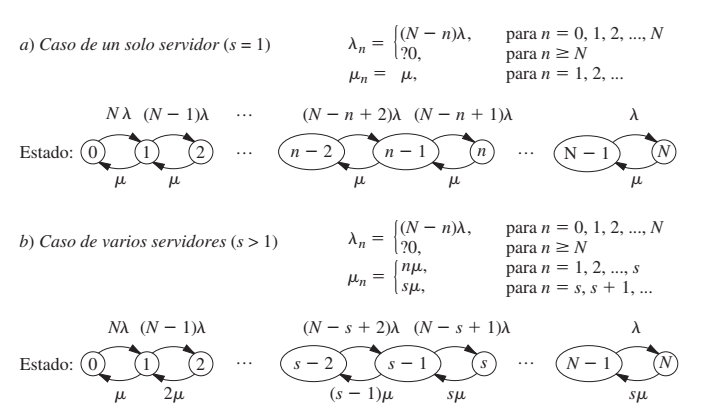
\includegraphics[width=0.9\textwidth]{images/Modelo_mm1n.png}
\end{center}
\end{frame}

\end{document}
